%\documentclass[draft]{jyflluk}
\documentclass[final]{jyflluk}

% Tämä tiedostopohja käyttää biblatexia. JOM (6.3.2016)
\usepackage{graphicx}

\usepackage{caption}
\usepackage{subcaption}


% Variable "\Otsikko" in LaTeX
\newcommand{\Otsikko}{Microfluidic cancer cell sorting using dielectrophoresis}


%----------------------------------------------------------------------------------------
% LÄHDELUETTELON MUOTOILU
%----------------------------------------------------------------------------------------
\usepackage{csquotes}
\usepackage[backend=biber,style=nejm,sorting=none,maxnames=3,minnames=1,giveninits=true]{biblatex}
\usepackage{xcolor}


\addbibresource{source.bib}

%----------------------------------------------------------------------------------------
% KANSILEHDEN MUOTOILU JA TEKSTI
%----------------------------------------------------------------------------------------
\newcommand*{\titleJYFL}{\begingroup  % Create the command for including the title page in the document
\hbox{                                    % Horizontal box
\hspace*{0.1\textwidth}                   % Whitespace to the left of the title page
\rule{1pt}{\textheight}                   % Vertical line
\hspace*{0.05\textwidth}                  % Whitespace between the vertical line and title page text
\parbox[b]{0.8\textwidth}{                % Paragraph box which restricts text to less than the width of the page

% Tutkielman nimi
{\noindent\LARGE\bfseries \Otsikko\\[0.5\baselineskip]}\\[2\baselineskip]
%
% Tutkielman tyyppi ja päiväys
{\large Master's thesis, \today}\\[3.5\baselineskip]
%
% Tutkielman tekijä 
{\normalsize Author:}\\[0.5\baselineskip] 
{\large \textsc{Peter Balogh}}\\[1\baselineskip]
%
% Työn ohjaajat
{\normalsize Supervisor:}\\[0.5\baselineskip]
{\large \textsc{Andreas Johansson}}
%
% Tyhjä väli ohjaajan nimen ja yliopiston logon välille - älä poista seuraavaa tyhjää riviä!

\vspace{0.2\textheight}
% Yliopiston logo, nimi ja ainelaitos

\includegraphics[height=27mm]{JYU_LOGO.pdf} 
}
}        
\endgroup}
%----------------------------------------------------------------------------------------
% VARSINAINEN DOKUMENTTI
%----------------------------------------------------------------------------------------
\begin{document}
%----------------------------------------------------------------------------------------
% KANSILEHTI
%----------------------------------------------------------------------------------------
\titleJYFL

%----------------------------------------------------------------------------------------
% TIIVISTELMÄ
%----------------------------------------------------------------------------------------
\section*{Abstract}
\addcontentsline{toc}{section}{Abstract}

% Bibliografiset tiedot
Balogh Peter\\ 
\Otsikko\\
Master's Thesis\\ 
Department of Physics, University of Jyväskylä, 2020, \pageref{LastPage}~pages

\bigskip

\textbf{Some filler text, abstract will be done LAST}
\newline
% Tiivistelmän teksti
\noindent Heti opinnäytteen nimiölehden jälkeen sijoitettava tiivistelmä on yhdelle paperille mahtuva ja tavallisesti enintään 250 sanaa sisältävä yhteenveto, joka hyvin tiiviissä muodossa informoi kirjoituksesta. On tärkeää, että tiivistelmä laaditaan huolellisesti, koska sen välityksellä tieto kirjoituksesta leviää eri tietokantojen kautta. Sen tulee olla laadittu niin, että se sellaisenaan voidaan julkaista tietokannoissa. Tiivistelmään alkuun on merkittävä opinnäytteen bibliografiset tiedot ja sen lopussa mainitaan sitä kuvaavat avainsanat. Tiivistelmiä on kahta tyyppiä. Informatiivinen tiivistelmä on tärkein. Se kertoo, mitä ja miten on tutkittu ja mitkä ovat tulokset. Indikatiivinen tiivistelmä osoittaa, mitä kirjoituksessa on käsitelty. Se on sisällöltään yleisempi kuin informatiivinen tiivistelmä, eikä se kerro tuloksista. Tiivistelmän loppuun liitetään aihetta kuvaavat 3--5 avainsanaa helpottamaan tietokantajärjestelmien työtä. Avainsanat voidaan antaa vapaasti asiasisällön mukaan tai poimia termit alan kontrolloiduista sanastoista kuten Yleisestä suomalaisesta asiasanastosta YSA. Opinnäytteen tunnistamiseksi tarvittavat bibliografiset tiedot annetaan tiivistelmän alussa. Tarvittavat tiedot ovat kirjoittajan suku- ja etunimi, opinnäytteen otsikko, opinnäytteen tyyppi, ainelaitoksen nimi, yliopiston nimi, valmistumisvuosi ja työn sivujen lukumäärä (ilman liitesivuja).

\bigskip

% Avainsanat
\noindent Avainsanat: 

%----------------------------------------------------------------------------------------
%	ABSTRACT
%----------------------------------------------------------------------------------------
\section*{Tiivistelmä}
\addcontentsline{toc}{section}{Tiivistelmä}

% Bibliographic information
Peter Balogh\\
\Otsikko \\
Pro gradu -tutkielma \\
Fysiikan laitos, Jyväskylän yliopisto, 2020, \pageref{LastPage}~pages.

\bigskip

% Abstract text
\begin{otherlanguage}{english}
\noindent This should be written in English.
\end{otherlanguage}

\bigskip 

% Keywords
\noindent Keywords: Thesis, abstract, writing, instructions

% --------------------------------------------------------------------------
% ESIPUHE
% --------------------------------------------------------------------------
\section*{Preface}
\addcontentsline{toc}{section}{Preface}

Esipuheen teksti tulee tähän.

\bigskip

Jyväskylässä "DATE HERE"

\bigskip

Peter Balogh

% --------------------------------------------------------------------------
% SISÄLLYS
% --------------------------------------------------------------------------
\tableofcontents

% --------------------------------------------------------------------------
% VARSINAINEN TEKSTIOSA
% --------------------------------------------------------------------------
\section{Introduction}
\label{sec:introduction}

Microfluidics is a field where systems operate with smaller quantities of fluids than nanolitre ($\SI{100}{\micro \metre}^3$). Working with such small volumes allows high speed and precise localisation for analysing small particles. Today, microfluidics is mainly used for molecular analysis, but it started off in the 1950’s being a part of ink jet printer manufacturing \cite{gervais_microfluidic_2011}. From there on microfluidics developed after the cold war to field-deployable systems for detection of biological and chemical hazards. In 1980 the rapid growth of molecular biology genomics pushed the development for high throughput DNA sequencing. Finally, the development of the silicon microelectronics contributed with their influence. Photolithography methods could be used to used for microfluidics which allowed further complexity being added on chips, such as electronical detection mechanisms. \cite{whitesides_origins_2006}

Microfluidics give the possibility for cell separation and analysis. Resulting from the small volumes, laminar and high flow speed is achievable. Thus, single cells can be guided through channels and analysis with a high throughput. One important application for this is the separation of individual cancer cells from blood. For cancer treatment, thorough analysis of the cells is required to find out which drugs can work on the specific cancer of an individual. The cells could be screened from blood thus requiring no physical operation, which is important for tumours in difficult areas (e.g. the brain). Fast sorting is required because of their low concentration in blood, circulating cancer cells can be as rare as one in $10^8$ blood cells \cite{huang_enrichment_2013}. This sets the requirement fast analysis; the throughput should be over the kHz range to be practical. 

There are multiple ways for sorting and detecting cells. Optical, thermal, chemical, acoustic, mechanical, magnetic and electrical techniques have been used for cell sorting \cite{ahn_dielectrophoretic_2006,zhang_towards_2015, voldman_electrical_2006}. To differentiate between cells their intrinsic properties, such as size, refractivity or electrical properties can be exploited. One method is to label a cell with a biological marker.  For example, an antibody attached to a fluorophore can label specific proteins or cells selectively. The availability of various biological labels allows cells to be differentiated by fluorescence, radioactivity or by a change in their electromagnetic properties \cite{wilhelm_universal_2008}. Dielectrophoresis is a phenomenon where a force can be exerted on a polarisable particle using a non-uniform electric field. It allows control of unlabelled cells and is the one the fastest sorting methods \cite{zhang_towards_2015}.

A highly popular method for microfluidic device fabrication is “soft lithography”. It includes the use of polymers such as Polymethylsiloxane (PDMS) to create mold of microstructures. Although it is an inexpensive and fast method capable of creating complex structures like valves and pumps, it has its limitations \cite{xia_soft_1998,tian_introduction_2009, pethig_review_2010, grover_monolithic_2003}. PDMS can swell because of organic solvents and be damagaed \cite{lee_solvent_2003}. Polymers also have limited chemical, mechanica and thermal resistance. In addition, they restrict low waveleght light ($\SI{400}{\nano \metre}$) required for laser induced fluorescence spectroscopy \cite{tian_introduction_2009,stankova_optical_2016}. Amongst the huge spectrum of microfluidic devices, rarely in a pure glass device is manufactured because of soft lithography methods being much easier and cheaper. Glass based microfluidics have three main advantages in biological analysis, they are chemically thermally and mechanically stable and are transparent in the visible light wavelength region. The mechanical stability allows to create high pressure, thus hight throughput systems. The chemicals stability together with thermal stability allows various solvent usage and cleaning possibility of clogged devices for repeatable use \cite{ofner_high-throughput_2017}. The isolating and heat dissipation properties of glass also allow for high-voltage and frequency dielectrophoretic sorting \cite{effenhauser_high-speed_1994}.
Sorting cells with a $100 \percent$ accuracy \cite{takahashi_non-destructive_2004, thomas_imagebased_2019} or high throughput methods \cite{zhang_towards_2015} have been developed in the past. Sciambi and R.Abate have even manufactured a device capable of $\SI{30}{\kilo \Hz}$ sorting with $>99 \percent$ accuracy. Regardless, high speed together with $100\percent$ accuracy has not yet been shown.

Dielectrophoretic droplet sorting in a glass device has been demonstrated by Ján Borovský for sorting carbon nanotubes at a femtolitre scale \cite{borovsky}. The aim in this thesis is to upscale such a device to be capable of single cell, high throughput, dielectrophoretic sorting. It would be the a part of a microfluidic chip complex, where cells are pre-sorted to higher concentrations using inertial sorting (capable of sorting $\num{3e8}$ cells/s \cite{edd_microfluidic_2020}) and then individual sorting done with dielectrophoresis. Here, the process of fabrication is developed to realise a microfluidic chip suitable for dielectrophoretic sorting using fluorescence spectroscopy. The process is conducted using basic microfabrication methods; e-beam lithography, thin film evaporation, and wet etching.



%%%%%%%%%%%%%%%%%%%
%%%%%%%%%%%%%%%%%%%
%%%%%%%%%%%%%%%%%%%
\section{Theoretical background}
\label{sec:theoretical_background}

There are three main sections of theory, they shall be devided into subsections once suitable subjects has been found.

\subsection{Microfluidics}
\label{sec:subsection1}
\begin{itemize}
    \item  How microfluidics differs from normal fluidics?
    \item  What are the main dimensions/ phenomena affecting microfluidics? 
    \item  Picolitre vs femtolitre, laminar flow, possibilities for high current-> fast analysis
    \item  Some equations? 
\end{itemize}




\subsection{Cell sorting}
\label{sec:x2}
 \begin{itemize}
     \item Imortance of single cell (cancer) sorting
     \item Labeling and detecting cells (fluoresence, radioactive, magnetic?(nanobeads?)
     \item Different methods for sorting (inertia, dielectrophoresis, electrophoresis, labels etc...
 \end{itemize}

\newpage
\subsection{Dielectrophoresis}
\label{sec:x3}
\subsubsection{Theory}
\label{sex:x3.1}

Dielectrophoresis (DEP) is a phenomenon, where a non-uniform electric field can cause a force on a polarizable particle. This phenomenon can be used to move and separate label-free particles. A uniform electric field would cause a uniform charge-distribution on an polarizable particle therefore creating a net-force equal to zero. Respectively, a non-uniform electric field will cause the positive and negative charge accumulation inside the particle to be uneven, causing a net force (Figure \ref{fig:DEP1}b). The direction and the magnitude of the force will depend on the particle’s and mediums polarizability and the electric field \cite{shafiee_contactless_2009}. The term dielectrophoresis was already introduced in 1951 by Herbert A. Pohl \cite{pohl_motion_1951}. It has since gained popularity in microsystems because of its simplicity and favourable scalability $F_{dep} \propto V^{2}/L^{3}$. Here $V$ is the applied voltage and $L$ the distance from particle to electrodes. Meaning, on a smaller system, less voltage is required to achieve the same force $F_{dep}$ \cite{castellanos_electrohydrodynamics_2003}.
\begin{figure}[h]%
    \centering
    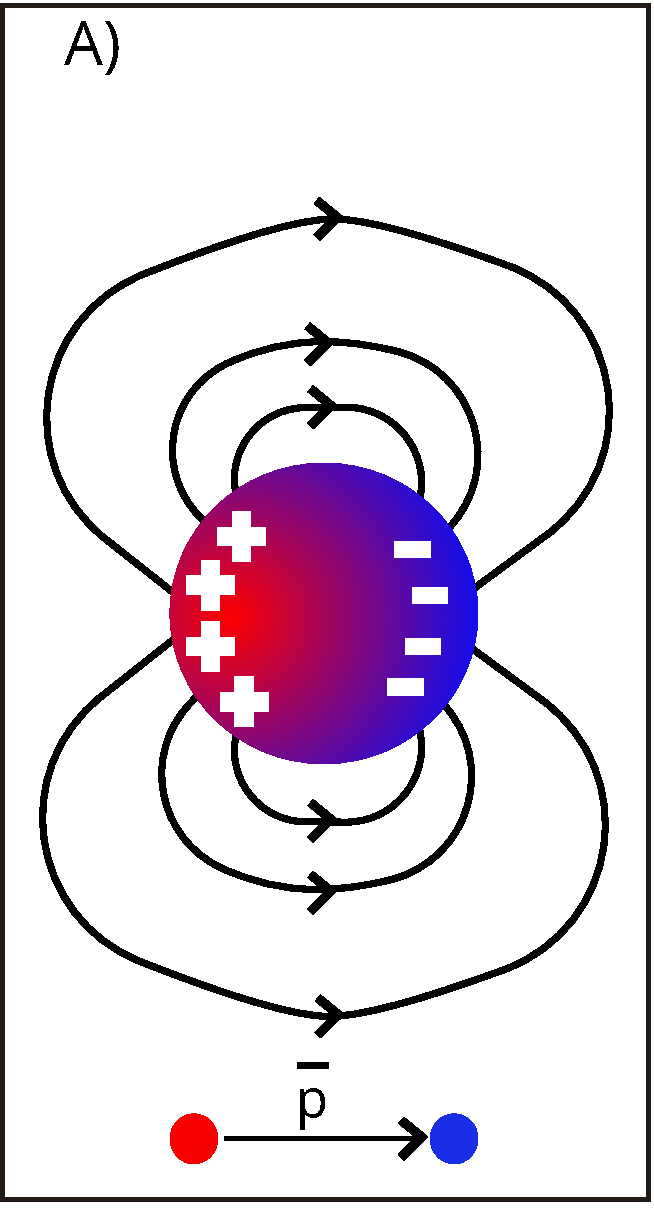
\includegraphics[width=.32\linewidth]{images/pooolar.pdf}\quad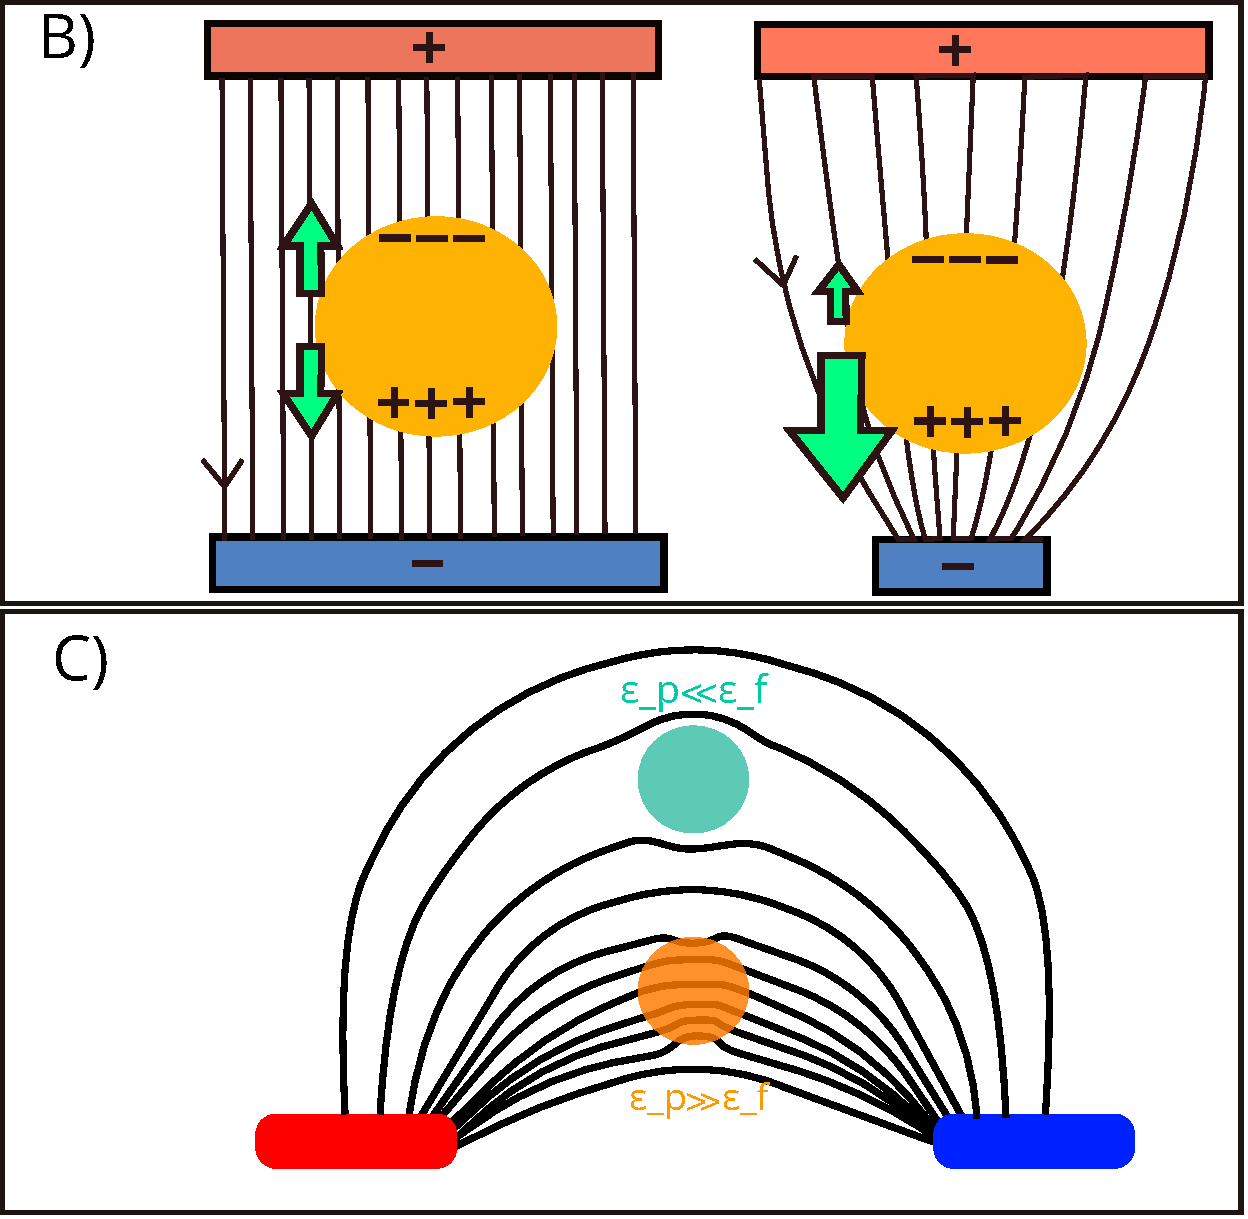
\includegraphics[width=.61\linewidth]{images/merged.pdf}
    \qquad
    \begin{minipage}{1.2in}
    \end{minipage}%
    \caption{Visualisation of DEP. A) A Polarised spehere has a dipole moment B) Net force in a uniform and non-uniform electric field C) Particle and medium permitivity effect on electric field }%
    \label{fig:DEP1}%
\end{figure}

There are multiple mathematical models describing DEP \cite{jubery_dielectrophoretic_2014}. They vary on their complexity and demand on computational power. Here we will be presenting a simplified and general method for the DEP force calculations which has been presented by a number review articles \cite{cottet_mydep_2019, morgan_single_2007,li_review_2014,voldman_electrical_2006}. The force experienced by a dielectric particle can be expressed as
%
\begin{equation}
   \label{eq:F_dielec}
   \vec{F}_{\mathrm{DEP}} = \vec{p} \vec{\nabla} \vec{E}\;,
\end{equation}
%
where $\vec{p}$  is the dipole moment vector, and $(\vec{\nabla} \vec{E})$ the gradient of electric field. The dipole moment depends on the shape of the particle, for a perfect dielectric uniform sphere, it can be expressed as
%
\begin{equation}
   \label{eq:dipmoment}
   \vec{p} = 2 \pi \epsilon_f R^3 \mathrm{Re}[f_{CM}] \vec{E}\;,
\end{equation}
%
Here $R$ is the radius of the particle, $\epsilon_{f}$ the absolute permittivity of surrounding fluid and $\mathrm{Re}[f_{CM}]$ the real part of the Clausius-Mossotti factor (CM) \cite{li_review_2014}. The CM factor for a spherical particle is
%
\begin{equation}
   \label{eq:CM}
   f_{CM} = \left(\frac{\epsilon_{p}^* - \epsilon_{f}^*}{\epsilon_{p}^* + 2\epsilon_{f}^*} \right)\;,
\end{equation}
%
Where and $\epsilon^*$ the complex absolute permittivity of the particle (p) and the surrounding fluid (f). They are related to conductivity $\sigma$ and the angular frequency $\omega=2\pi f$ of the electric field as 
%
\begin{equation}
   \label{eq:complex}
   \epsilon^* = \epsilon - \frac{i \sigma}{\omega}\;,
\end{equation}
%
$i$ being $\sqrt{-1}$. Combining equations (1) and (2) we get and expression for the force
%
\begin{equation}
   \label{eq:F_DEP_norm}
   \vec{F}_{\mathrm{DEP}} = 2 \pi \epsilon_f R^3 \mathrm{Re}[f_{CM}] \vec{\nabla} (\vec{E} \cdot \vec{E}) 
\end{equation}
%
For an AC potential the time average of the force can be expressed as
%
\begin{equation}
   \label{eq:F_DEP}
   \langle F_{\mathrm{DEP}}\rangle = 2 \pi \epsilon_f R^3 \mathrm{Re}[f_{CM}] \vec{\nabla} (E^2_{RMS}) ,
\end{equation}
%
where $E_{RMS}$ is the root mean square value of the electric field $E=\mathrm{Re}[E_0 e^{i \omega t}]$. When the CM factor is expanded (Eq.\ref{eq:complex}) we can see the frequency dependence.
%
\begin{equation}
   \label{eq:CM_open}
   f_{CM} = \left(\frac{(\epsilon_{p} - \epsilon_{f}) + \frac{i}{\omega} (\sigma_f - \sigma_p)}
   {(\epsilon_{p} + 2\epsilon_{f}) - \frac{i}{\omega} (\sigma_p - 2\sigma_f)} \right)\;
\end{equation}
%
Examining the electric field at low  $(\omega = 0)$ or a high frequencies $(\omega = \infty)$ we can see that the CM is reduced to 
\begin{equation}
   \label{eq:wat0}
   f_{CM} = \frac{\sigma_p - \sigma_f} {\sigma_p + 2\sigma_f}, \; \mathrm{when } \;\omega \rightarrow 0 \;
\end{equation}
\begin{equation}
   \label{eq:watinf}
   f_{CM} = \frac{\epsilon_p - \epsilon_f} {\epsilon_p + 2\epsilon}, \;\mathrm{when } \;\omega \rightarrow \infty\;
\end{equation}





At high frequency, the particle acts like a capacitor and is dominated by its permittivity. Whereas, at very low frequencies the current in the particle moves in phase with the electric field thus the conduction is the dominating factor \cite{cetin_dielectrophoresis_2011, li_review_2014, pethig_review_2010}. 
From the CM factor (Eq.\ref{eq:CM}) we can also see that the permittivity of the particle and the surrounding medium determines whether force is pushing or pulling towards the region of stronger electric field. If the particle is more polarizable $(\epsilon_p>\epsilon_f)$ a positive force (pDEP) is pushing towards he higher field and vice versa (Figure \ref{fig:DEP1}c). We can also see from $\epsilon_p>>\epsilon_f$ and  $\epsilon_p<<\epsilon_f $ that the positive DEP force (pDEP) can be twice the magnitude of the negative DEP force (nDEP).
The most important points arising from these equations are:

\begin{enumerate}
\renewcommand{\labelenumi}{\roman{enumi}}  % <<<<<<<<<<<
    \item The Force is zero in a uniform field $(\nabla E=0)$.
    \item The force depends non-linearly on the field magnitude $(E^2)$ and showing that both an AC and CD field can cause a DEP force.
    \item The dependence on particle volume $\propto R^3$ allows separation of particles based on size.
    \item Due to conductivity and permittivity dependence of the medium and particle, the DEP force can be pulling or  pushing. By changing the frequency, there is a crossover-frequency where pDEP changes to nDEP can be achieved. \cite{zhang_dielectrophoresis_2010}
\end{enumerate}
The simplifications made when deriving Eq.\ref{eq:F_DEP} need to me taken into consideration. The particle needs to be a perfect homogeneous dielectric sphere with no net charge. The particles polarisation is assumed as a simple dipole moment, even though a non-uniform field is causing the polarisation.  The medium around the particle is considered infinite, and not affected by the particle itself. \cite{pethig_review_2010}
In our study, we are aiming to use DEP to sort cells. They have various shapes and are not uniform. Cells contain membranes, cytoplasm and organelles. In order to have higher accuracy for simulations more precise mathematical models can be introduced at the cost of computational time \cite{jubery_dielectrophoretic_2014, cetin_dielectrophoresis_2011, pethig_review_2010, cottet_mydep_2019}. But, even with the simplifications, this model is sufficient to describe the our DEP system because the underlying physics are present.

\textcolor{red}{!more specific calculations are availavable? Should i?}
\subsubsection{Single shell model}
\label{sec:x3.2}

The CM factor for a mammalian cell has characteristic properties. For example, a white blood cell has been demonstrated \cite{voldman_electrical_2006}. At low frequencies ($<\SI{100}{\kilo \Hz}$) the cell is less polarizable than a typical ionic solution thus causing a nDEP effect. Similarly when going to Mhz frequencies, the conductivities of the solution and the cell will matter more, thus resulting in a pDEP in low conductivity solutions ($\SI{5.5e-6}{ \siemens \per \metre}$ for Di water \cite{pashley2005gassed}). At GHz range, the the permitivities will me mainly compared (Eq.\ref{eq:watinf}) and likely to cytoplasmic proteins, the permittivity of the cell is low compared to water and results in a negative dep.  Although the frequency depends highly on the cell and medium properties, the “single-shell” model (Figure \ref{fig:single_shell}) predicts this two times cross over frequency \cite{cetin_dielectrophoresis_2011,pethig_review_2010, voldman_electrical_2006, cottet_mydep_2019}. The single-shell model uses a CM factor where a shell (cf. cell membrane) is accounted for with its own properties. In the single shell model the complex permittivity is
%
\begin{equation}
   \label{eq:shellmodel}
   \epsilon^*=\epsilon_{mem} \left[ \frac{\left( \frac{r}{r-d}\right)^3 + 2\left(\frac{\epsilon_{CP}^* - \epsilon_{mem}^*}{\epsilon_{CP}^* + 2\epsilon_{mem}^*} \right)}{\left( \frac{r}{r-d}\right)^3 -\left(\frac{\epsilon_{CP}^* - \epsilon_{mem}^*}{\epsilon_{CP}^* + 2\epsilon_{mem}^*} \right)}        \right] \;,
\end{equation}
%
where $r$ , $d$ the thickness of the membrane, $\epsilon_{CP}^*$ and  $\epsilon_{mem}^*$ are the complex permitivities of the cytoplasm an the membrane. A simulation of the CM factor using the single shell model for HT-29 cells is shown in Figure \ref{fig:single_shell}. The result is from a Java  simulator published by Cottlet et Al \cite{cottet_mydep_2019}.

\begin{figure}[h]%
    \centering
    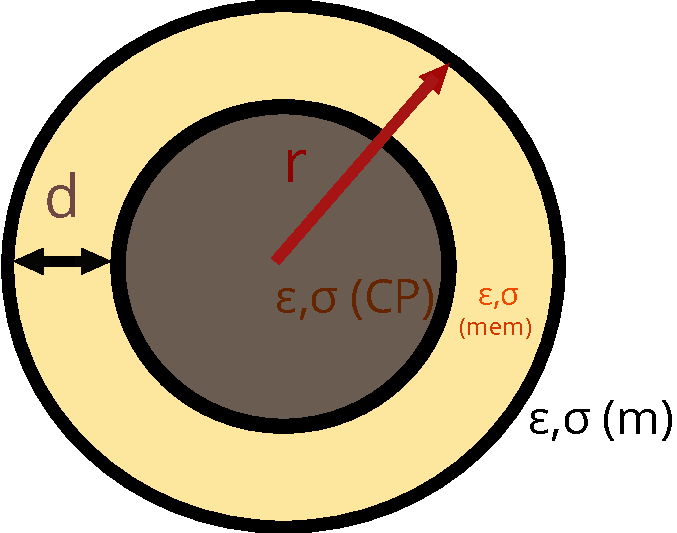
\includegraphics[width=.27\linewidth]{images/single_shell.pdf}\quad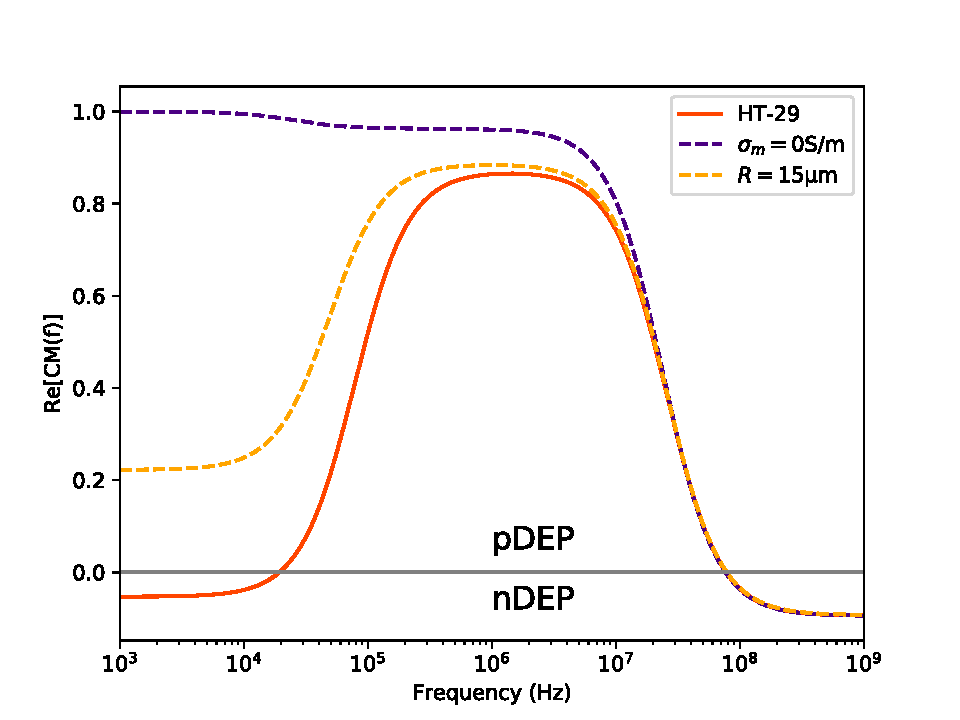
\includegraphics[width=.61\linewidth]{images/plot_DEP.pdf}
    \qquad
    \begin{minipage}{1.2in}
    \end{minipage}%
    \caption{(Left) Single shell modell, (Right) CM factor for Human colon cancer cells (HT-29) has been simulated with MyDEP tool \cite{cottet_mydep_2019}. The values used in the simulation are presented in table \ref{tab:cell_table}. A change in cell radius and a change in media was also simulated for comparison.}%
    \label{fig:single_shell}%
\end{figure}


For comparison, a simulation was also done with the same cell having a larger radius and one being submerged in DI-water $(\sigma_{DI}\approx0)$. In reality, the change in medium conductivity can affect the membrane conductivity up to 2 orders of magnitude, which has not been accounted for in this simulation \cite{wu_dielectrophoretic_2012}. This simulation gives a sense for order of magnitude of the frequency to be used in our experiment. It also shows that cells with different properties, such as size, electrical properties and shape, can be separated with DEP with a correct frequency. Around the crossover frequency cells can experience nDEP or pDEP depending on their properties. Separating cancer cells from blood using DEP has already been demonstrated by multiple publications \cite{becker_separation_1995,huang_enrichment_2013,kang_continuous_2006, ivory_direct_2011}.

\begin{table}[h]
   \centering
   \caption{The literacy values for HT-29 Human colon cancer cells \cite{wu_dielectrophoretic_2012}.}
   \label{tab:cell_table}
   \begin{tabular}{cccccc} \toprule
      $\sigma_m$ (S/m)    & $\epsilon_{mem}$ & $\epsilon_{mem}$ & $\sigma_m$ (S/m) & $\sigma_m$ (S/m) & $R$ ($\mathrm{\micro\metre})$\\ \midrule
      $0.01$              &  $4.68$        &  $68.31$       & $6.63e-6$        & $0.279$          & $6.6$\\
        \bottomrule
   \end{tabular}
\end{table}


\subsubsection{Choosing DEP}

For successful high throughput cell sorting, the correct parameters are needed to be chosen to our DEP system by accounting for all the problems and advantages. The electrodes for DEP can be manufactured to be in contact with the sample fluid or contactless. DEP can be achieved using AC or DC currents. The field strength can be chosen by varying the potential or the dimensions of the electrodes. For nDEP or pDEP the correct frequency needs to be chosen for the AC alternative. As an outcome, the DEP force needs to outscale drag force, buoyancy force, electrothermal forces and Brownian motion (not a problem for >1um particles) \cite{cetin_dielectrophoresis_2011}.
For DEP applications, the most common way is placing the electrodes in contact with the liquid. This allows the particles to be closer to the electrodes thus perceiving a higher gradient allowing higher precision control \cite{voldman_electrical_2006}. Unfortunately, contact with the sample fluid can lead to many problems, especially with biological samples. Electrode polarization, bubble formation, dissolution of electrodes, contamination of the fluid and fouling can affect the operation. Especially in DC systems electrochemical effects can produce $\mathrm{H_2}$ and $\mathrm{O_2}$ gas. Joule (resistive) heating causes a problem, already $>4\celsius$ above body temperature ($37\celsius$) can lead to mammalian cell death. \cite{voldman_electrical_2006,cetin_dielectrophoresis_2011,shafiee_contactless_2009}.
Using contactless electrodes, bubble formation, contamination and  fouling are completely eliminated. The medium is then only in contact is the substrate. This also reduces heating from a high intensity light, e.g. Fluorescence inducing light, absorbed by the electrodes. For contactless electrodes AC is the better choice, because DC would require higher voltages for sufficient DEP, which lead to joule heating. A high frequency electric field is also less stressing on a cell membrane, which have voltage sensitive proteins, than that of a DC field \cite{voldman_electrical_2006}.























































%%%%%%%%%%%%%%%%%%%%%%%%%
%%%%%%%%%%%%%%%%%%%%%%%%%
%%%%%%%%%%%%%%%%%%%%%%%%%


\section{Methods}
\label{sec:methods}

Here I present all the relevant methods for the fabrication process. FOr each, a short theory section including (HOW, WHAT HAPPENS, RESULT). Visualisations with a vector software (not decided). Equations  nescessary to illustrate the phenomena and important factors

\subsection{Cleaning and activation}
\label{sec:xx1}
RCA-cleaing basics. Acetone+IPA, sonication, mechanic scrubbing, Cleanroom etiquettes for low particle contamination,
DH2O. Pirahna solution explained (cleaning \& activation [activation by RIE menitioned])

\subsection{Mask evaporation}
\label{sec:xx2}
Theory, possibilities for mask deposition (short), E-BEAM evaporation, pros and cons (Defects), IMAGES!!

\subsection{Resist exposure and development}
\label{sec:xx3}
Small intro to litography, E-beam litography, Choosing right resist and spin speed, Exposure, IMAGES!!

\subsection{Wet eching}
\label{sec:xx4}
\begin{itemize}
    \item Basics of wet etching, isotropy etc...
    \item Etching of metals, especially Cr, Au
    \item Etching of glass
\end{itemize}


\label{sec:xx5}
\subsection{RIE}
\begin{itemize}
    \item Rie theory/ how it orks
    \item Usage for cleaning
    \item Usage for activation
    \item Usage for etching (we do etch SiO from electrodes :)
\end{itemize}

\subsection{Glass bonding}
\label{sec:xx6}
Thermal bonding explained, also chemical reaction Images. Requirements for a succesful bonding (how close glasses need to be, what surface activation etc..)


%%%%%%%%%%%%%%%%%%%%%%
%%%%%%%%%%%%%%%%%%%%%%
%%%%%%%%%%%%%%%%%%%%%%
\section{Fabrication}
\label{sec:fabrication}

PENDING: Wether to put electrodes first (as in fabrication) or channels

\subsection{Design}
\label{sec:xxx1}
The chip layout was designed using the electron microscopes own software (\textcolor{red}{Raith e-Line 150 ver. 5.0???}). There were two main considerations for the design; The important features required for the chip operation needed to be implemented and it needed to be simplistic allowing a low exposure time. When developing the fabrication steps, it is important to that all the features required can be produced, once the fabrication steps are mastered, the don’t need to be altered when changing the chip design. The most important features were the channels ranging between a depth of $(2-40) \mathrm{\micro \metre}$, a width of $(10-120) \mathrm{\micro \metre}$ and the manufacture of electrodes close as possible to the channels. E-beam was chosen as the lithography method for development to allow fast changes in design if necessary, without the need to create new masks as in photolithography. E-beam exposure time increases with area exposed, which had to be minimized for efficient development. 

The three most important areas of the channel layout are visualised in Figure \ref{fig:design1}. A) The channels from the two inlets meet at a T-crossing. It allows droplet formation, if droplet-based sorting is to be used, or flow control. If cells are inserted from one of the inlets, the space/medium between the cells can be altered by tuning the second inlet pressure to cause a stationary or a high-speed flow. This flow adds medium in between the cells thus increasing the distance between them. B) Is a straight line starting with normal width expanding into a long and wide channel. !!!!\textcolor{red}{At the start the cells would be better confined serving as a place for spectroscopy analysis!!!!(UNSURE)}. At the wider part the flow would slow down due to higher volume, and the electrodes placed next to the channel would exert either a pushing or pulling force the cells. Assuming a laminar flow, the cells would then take the correct “lane” in the wide channel to be then sorted. C) At the Y-junction the cells would go left or right depending on their “lane” to be collected or to become waste (Figure \ref{fig:design_flow}). The junction would also require small channels where cells don’t fit across to stabilize pressure. A cell going in right channel would then increase the drag on the fluid thus causing the left channel to be more favourable for the next incoming cell independent of its lane.

\begin{figure}
    \centering
    \begin{subfigure}[ht]{0.48\textwidth}
        \centering
        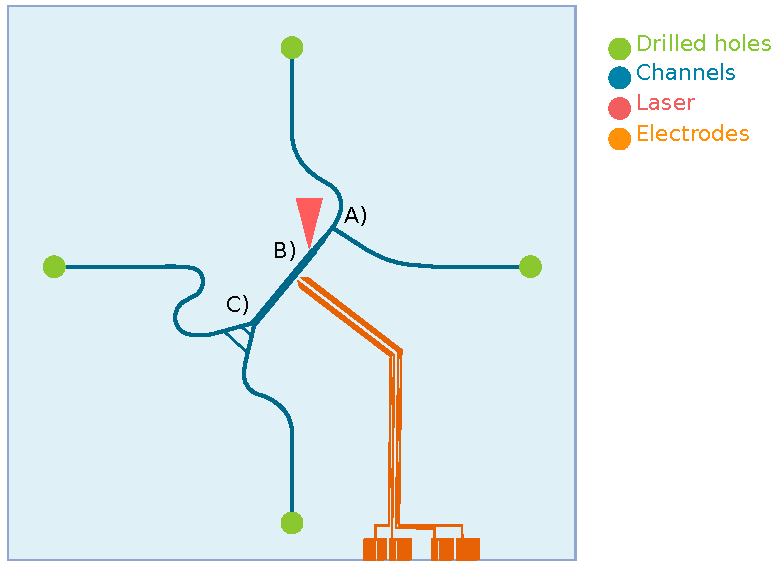
\includegraphics[width=\linewidth]{images/chip_design.pdf} 
        \caption{Chip layout.} \label{fig:design1}
    \end{subfigure}
    \hfill
    \begin{subfigure}[ht]{0.48\textwidth}
        \centering
        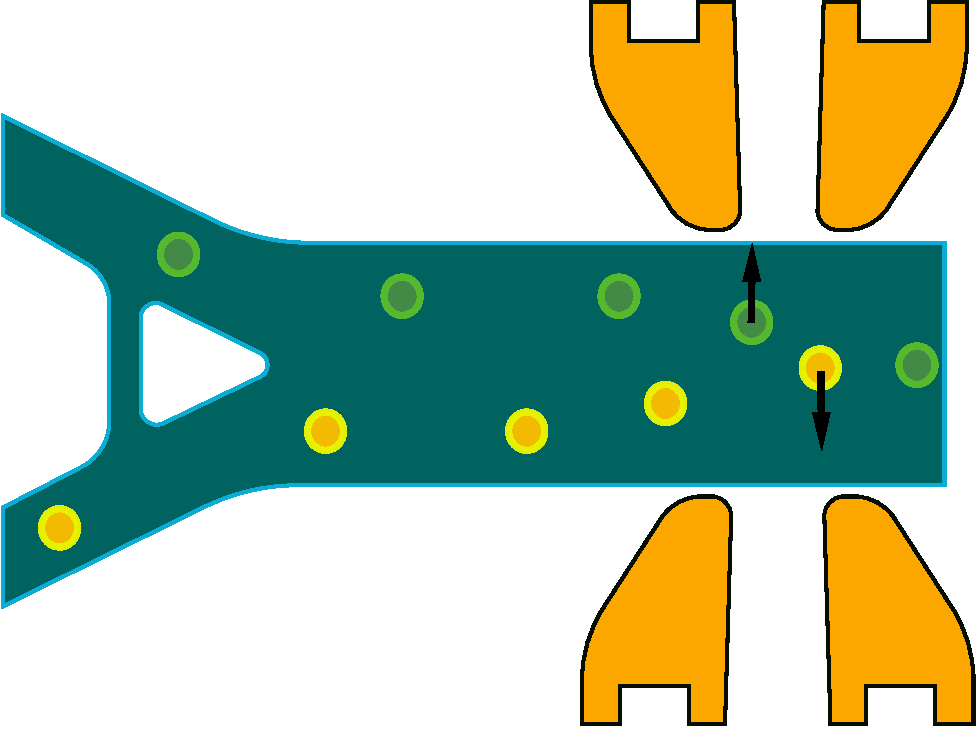
\includegraphics[width=\linewidth]{images/Separation.pdf} 
        \caption{Deflection of cells to different lanes} \label{fig:flow1}
    \end{subfigure}
    \caption{The design for the layout of the microfluidic chip.} \label{fig:design_flow}
\end{figure}  



The layout was designed for a chip of $20x20 \milli \metre$, where the two inlets and two outlets were each $\SI{7}{\milli \metre}$ from the chips centre point (Figure \ref{fig:design1}).  The channels were designed to curve smoothly without rough edges and shapes to uphold laminar flow and reduce clogging. The channel width was \textcolor{red}{??50um??} for the transport of cells \textcolor{red}{(size ??-??)} and 5um for the pressure stabilizing channels. At the electrodes, the channel width was up to 100um to allow proper flow lanes for the cells. The width on the design needed to accommodate for isotropic etching. The channels were always wider than the exposed width. The increase is discussed in chapter \textcolor{red}{(?? WET ETCHING??))}. Knowing the correct width was critical in placing the electrodes close as possible. Concerning the length, the straight part in front of the electrodes needs to be long enough for the spectroscopy and the separation to take place. The inlet channels before the T-junction and the outlet channels after the Y-junction were designed to have matching lengths. Especially for the outlets it is essential because otherwise there would be a pressure difference that would make one channel more favourable for the flow.

The design for the electrodes were reproduced for Borovsk’s thesis \cite{borovsky}. The tip shape originated from a paper by, where the electric fields were simulated to produce an ideal electric field for contactless DEP \cite{leman_droplet-based_2015}. The electrodes consisted of a half loop having contact pads at the end for allowing the test wether they were functional. The contact pads were split into vertical lines to reduce the exposure area and thus time significantly. The final optimal design would include uniform contact pads and four electrodes. If Same frequency pDEP or nDEP is to be achieved there need to be electrodes on both sides of the channel. For the process development only two electrodes were manufactured. 


\subsection{Overview of the process}
\label{sec:xxx2}

The realization of the microfluidic chip was performed with conventional micro-fabrication-methods. Varying steps and methods were tried through trial and error until success. The fabrication steps for a successful chip are shown in Figure \ref{fig:processFULL}.
1) Drilled Soda Lime-glass microscope coverslips are used as substrate. The glass chip is first cleaned \textcolor{red}{(section)} and treated with Piranha-solution prior to evaporation. 2) Using E-beam evaporation, a of $\SI{100}{\nano \metre}$ Cr thin film is evaporated to act as an etch mask. Next, PMMA of about $\SI{250}{\nano \metre}$ is spun before e-beam exposure. 3) The electrode design is then exposed and developed. 4) The Cr-mask etched followed by a dip into HF-HCL (10:1) solution to etch shallow grooves for the electrodes. After etching, a RIE O2 etch was used to activate the glass and clean PMMA residue from electrode channels. 5) Electrodes are then evaporated; a metal sandwich of $\SI{10}{\nano \metre}$ Ti +$\SI{50}{\nano \metre}$ Au +$\SI{10}{\nano \metre}$ Ti +$\SI{100}{\nano \metre}$ $\mathrm{SiO}_2$). 6) Lift-off is then carried out and the Cr-mask etched away. 7) A tougher RIE O2 treatment is used to activate the glass surface and $\SI{50}{\nano \metre}$ Cr + $(150 + 150) \,\nano \metre$ Au is evaporated in an $45^{\circ}$ angle while the wafer is rotated ensuring deposition to the walls of the trenches. 8) Now $\SI{2.2}{\micro \metre}$ of PMMA is spun to cover the shallow channels of the electrodes completely. 9) Alignment, exposure, and development of the Channels-layout is performed. 10) The Au and Cr masks are etched followed by a 55s HF-HCL etch of the channels. After removing the e-beam resist the gold mask is removed by etching the underlining Cr. 11) Last, the chip and its cover are cleaned and activated in Piranha so can be bonded. The bonding is performed in a furnace at $\SI{85}{\celsius}$ for 2h. The bonded chip is then treared with a RIE oxide etch to reveal the electrode pads for soldering and the chip is ready.





\textcolor{red}{figureas at wrong page for now, NEEDS a fix}
%Make numbers in figures go 1,2,3 instead of a b c
\renewcommand{\thesubfigure}{\arabic{subfigure}}

\begin{figure}
    \centering
    \begin{subfigure}[ht]{0.48\textwidth}
        \centering
        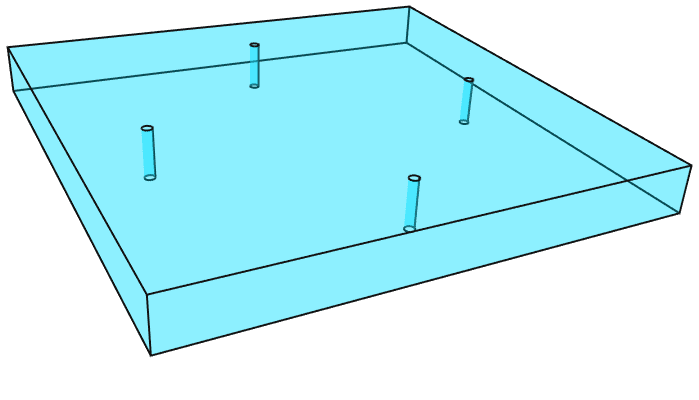
\includegraphics[width=\linewidth]{steps/1.Drilled.png} 
        \caption{Drilled Soda-lime glass chip} \label{fig:process1}
    \end{subfigure}
    \hfill
    \begin{subfigure}[ht]{0.48\textwidth}
        \centering
        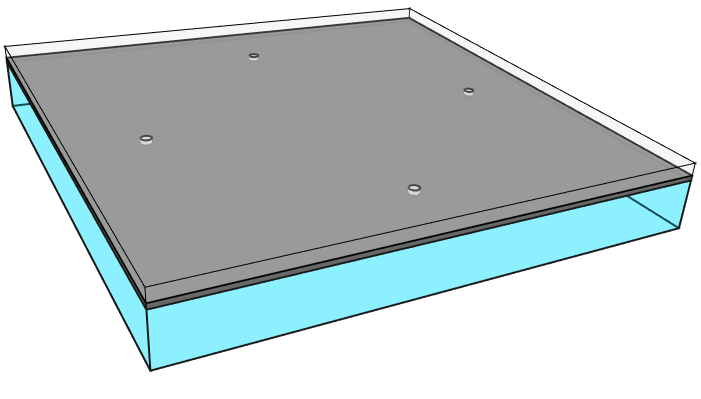
\includegraphics[width=\linewidth]{steps/2.Cr-Pmma.png} 
        \caption{$\SI{100}{\nano \metre}$ Cr + $\SI{250}{\nano \metre}$ PMMA} \label{fig:process2}
    \end{subfigure}
    
    \begin{subfigure}[t]{0.48\textwidth}
        \centering
        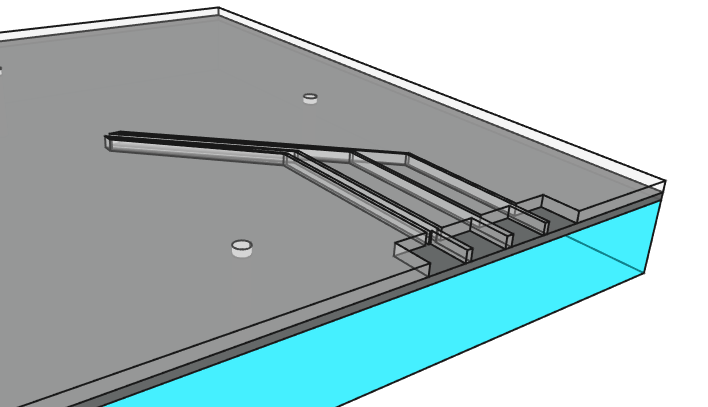
\includegraphics[width=\linewidth]{steps/3.Developed.bmp.png} 
        \caption{PMMA developed} \label{fig:process3}
    \end{subfigure}
    \hfill
    \begin{subfigure}[t]{0.48\textwidth}
        \centering
        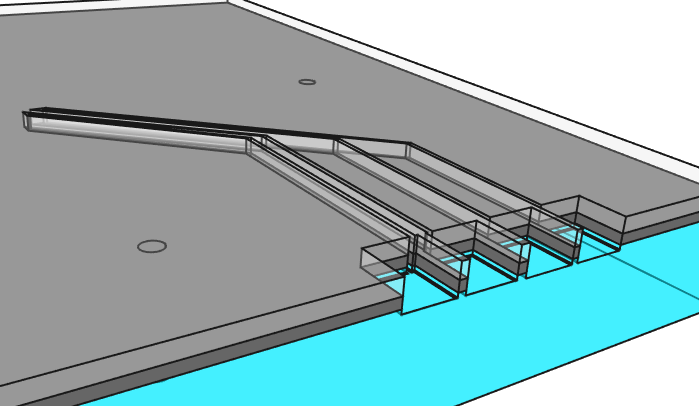
\includegraphics[width=\linewidth]{steps/4.Etched.png} 
        \caption{Cr-mask and Glass etched} \label{fig:process4}
    \end{subfigure}
    
    \begin{subfigure}[t]{0.48\textwidth}
        \centering
        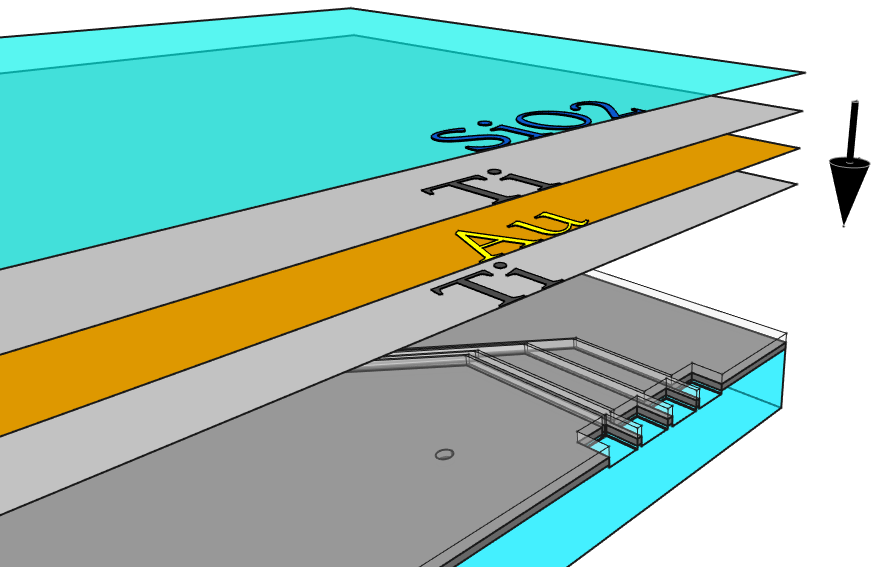
\includegraphics[width=\linewidth]{steps/5.-evap-Elec.png} 
        \caption{Electrodes deposited ($\SI{10}{\nano \metre}$ Ti + $\SI{50}{\nano \metre}$ Au + $\SI{10}{\nano \metre}$ Ti + $\SI{100}{\nano \metre}$ $\mathrm{SiO}_2$) } \label{fig:process5}
    \end{subfigure}
    \hfill
    \begin{subfigure}[t]{0.48\textwidth}
        \centering
        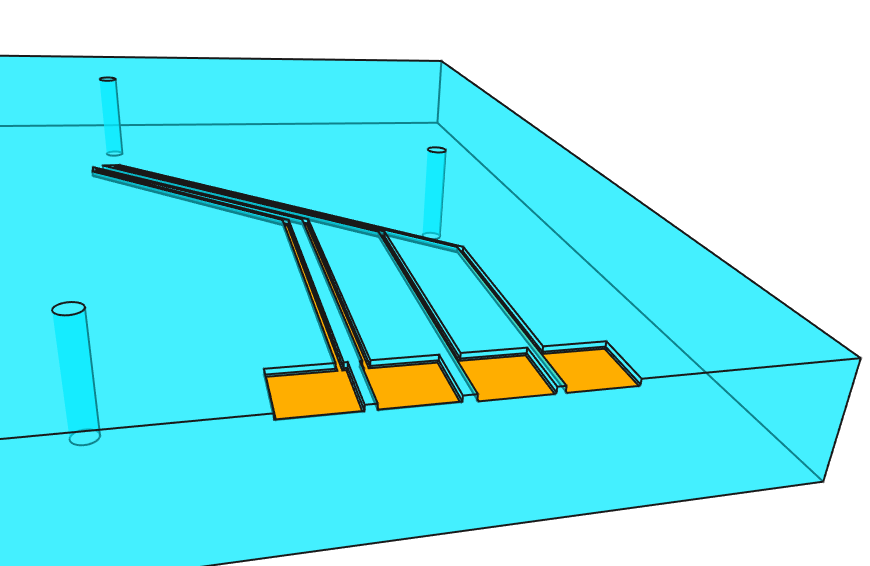
\includegraphics[width=\linewidth]{steps/6.-lift_off.png} 
        \caption{Lift-off} \label{fig:process6}
    \end{subfigure}
    
    \begin{subfigure}[t]{0.48\textwidth}
        \centering
        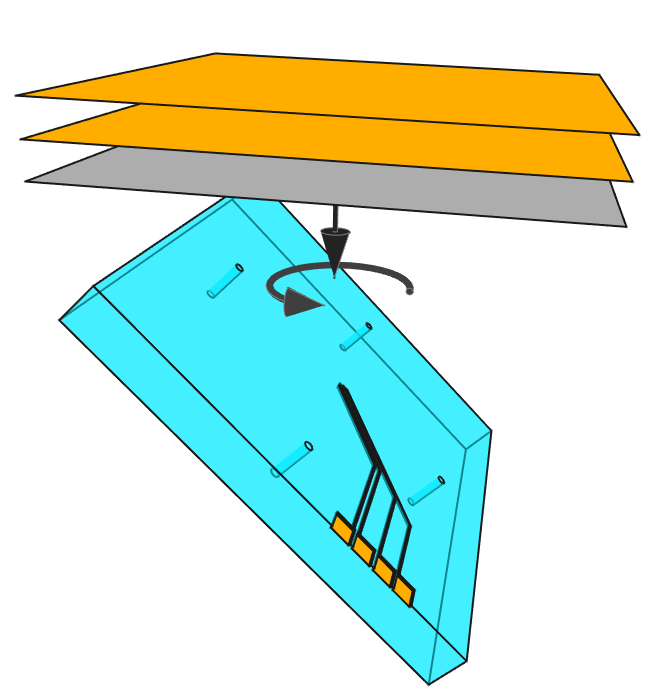
\includegraphics[width=\linewidth]{steps/7.evap_mask.png} 
        \caption{$\SI{50}{\nano \metre}$ Cr + $(150 + 150) \,\nano \metre$ Au deposited at $45^{\circ}$ angle on a spinning wafer} \label{fig:process7}
    \end{subfigure}
    \hfill
    \begin{subfigure}[t]{0.48\textwidth}
        \centering
        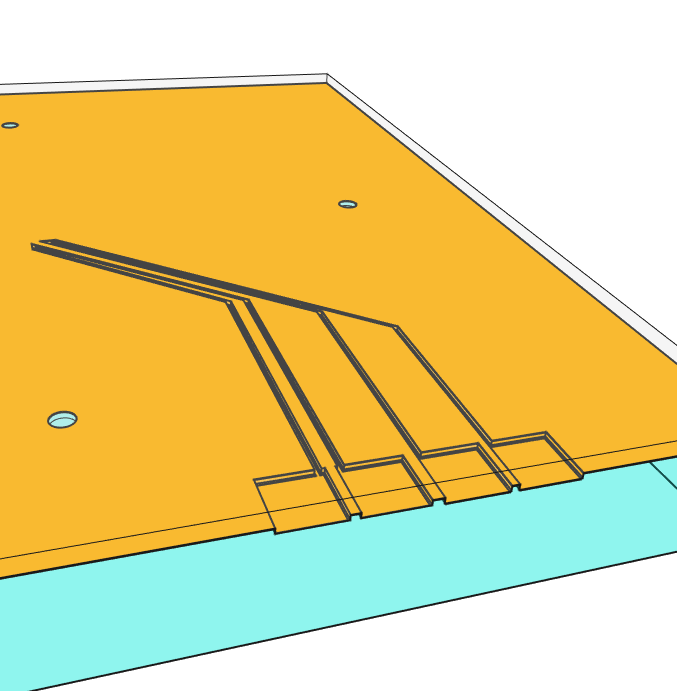
\includegraphics[width=\linewidth]{steps/8.pmma-thick.png} 
        \caption{$\SI{2.2}{\micro \metre}$ PMMA} \label{fig:process8}
    \end{subfigure}
\end{figure}  

%\captionsetup[subfigure]{labelformat=empty}
\begin{figure}\ContinuedFloat
    \centering    
    \begin{subfigure}[t]{0.48\textwidth}
        \centering
        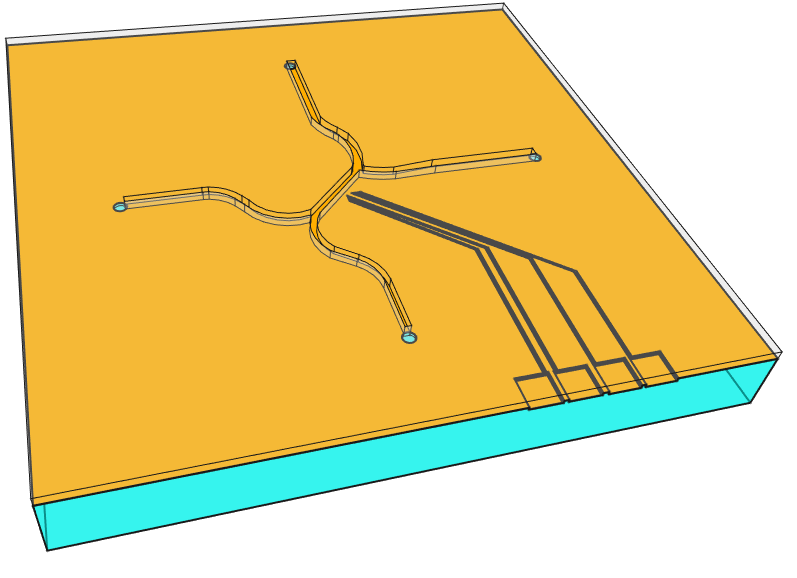
\includegraphics[width=\linewidth]{steps/9.developed2.png} 
        \caption{ Development} \label{fig:process9}
    \end{subfigure}
    \hfill
    \begin{subfigure}[t]{0.48\textwidth}
        \centering
        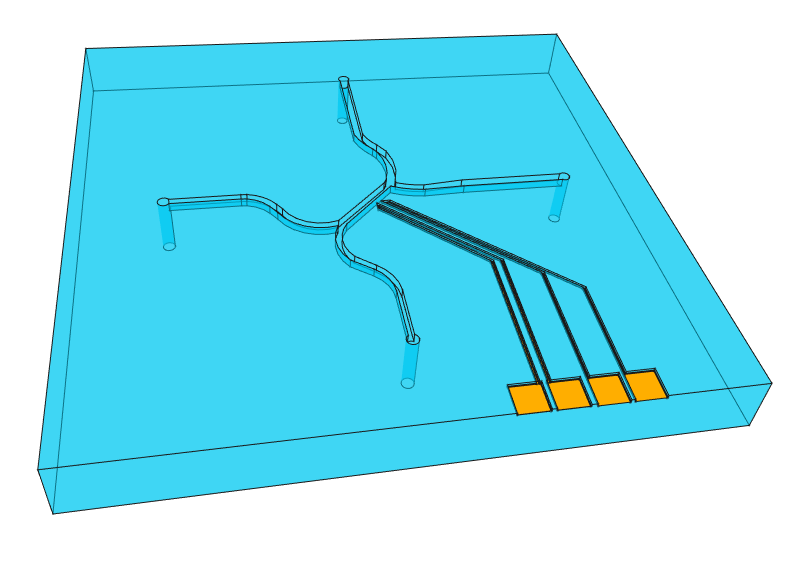
\includegraphics[width=\linewidth]{steps/10.etched.png} 
        \caption{Liftoff by etching Cr} \label{fig:process10}
    \end{subfigure}
    
    \vspace{1cm}
    \begin{subfigure}[t]{\textwidth}
    \centering
        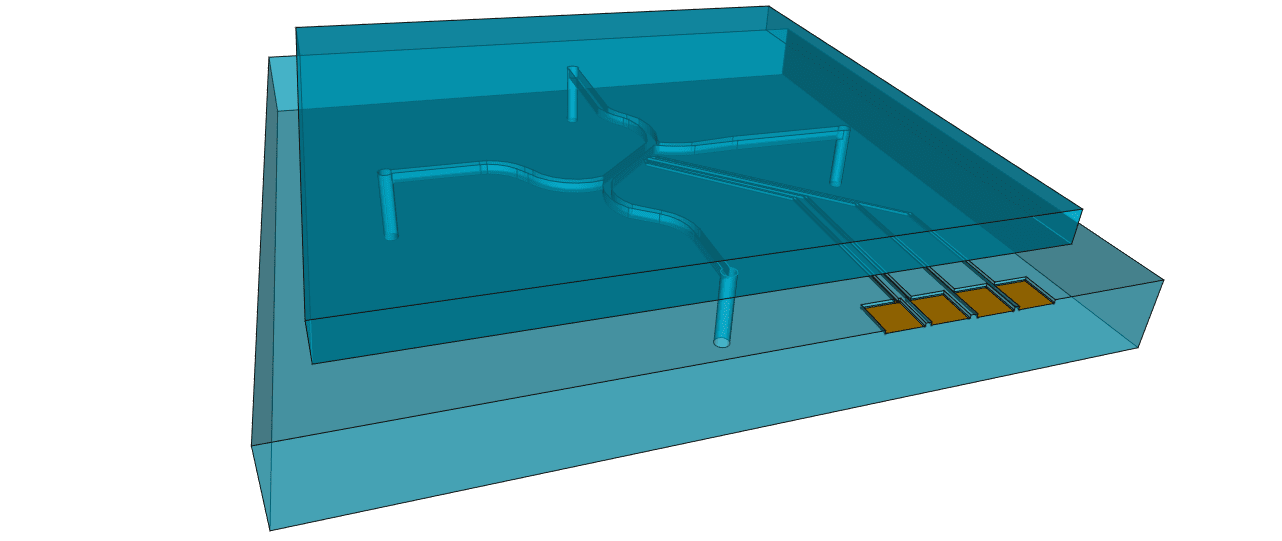
\includegraphics[width=\linewidth]{steps/11.Finished.png} 
        \caption{Thermally bonded cover} \label{fig:process11}
    \end{subfigure}
    \caption{The fabrication steps for a functional microfluidic chip} \label{fig:processFULL}
\end{figure}






\begin{itemize}
    \item images of all the steps in the correct order required to realise the chip
    \item short explanation of how the chip is manufactured
\end{itemize}







































\subsection{Channels}
\label{sec:xxx3}
\begin{itemize}
    \item Drillin of the holes (Missing info!)
    \item requirement for channels (depth, etc..)
    \item mask and wet etching
    \item images of progression in development, challenges that were faced
\end{itemize}

\subsection{Electrodes}
\label{sec:xxx4}
\begin{itemize}
    \item requirement for electrodes (material, withstand of pirahna, can take heat)
    \item mask and wet etching
    \item images of progression in development, challenges that were faced
\end{itemize}

\subsection{Experiment setup}
\label{sec:xxx5}
\begin{itemize}
    \item Microfluidic setup (images, and illustrative image of pressure pumping method)
    \item How the laser + high voltage was set-up (circuit diagram)
    \item images of progression, challenges that were faced
\end{itemize}



\section{Measurements (and results?)}
\label{sec:results}
\begin{itemize}
    \item flow speed (TO BE MEASURED)
    \item DEP setup, coltage and frequency tests, maby even elecrode distance (TO BE MEASURED)
    \item Deflection of fluorescent beads, maby even cells (TO BE MEASURED)
\end{itemize}


\section{Conclusions}
\label{sec:conclusions}

*** \textbf{Some example equations and references for latex} ***
\newline
Ideaalikaasun tilanyhtälön mukaan on komponentin $i$ osatiheys
%
\begin{equation}
   \label{eq:ideaalikaasun-tilanyhtalo}
   \rho_i = \frac{p_i M_i}{R T}\;,
\end{equation}
%
missä $p_i$ on komponentin $i$ osapaine ja $R$ on yleinen kaasuvakio. 

Komponentin $i$ mooliosuudelle $y_i = n_i/n$ saadaan yhtälöstä (\ref{eq:ideaalikaasun-tilanyhtalo}) Daltonin yhtälö
%
\begin{equation}
   \label{eq:daltonin-yhtalo}
   y_i = \frac{p_i}{p}\;.
\end{equation}

Koko seoksen tiheys ja kokonaispaine voidaan laskea vastaavasti kaavoilla~(\ref{eq:seoksen-tiheys}) ja (\ref{eq:seoksen-kokonaispaine}).

\begin{eqnarray}
   \rho & = & \sum_i \rho_i \label{eq:seoksen-tiheys} \\
   p & = & \sum_i p_i \label{eq:seoksen-kokonaispaine}
\end{eqnarray}




Tulokset esittelee ja kommentoi tutkimuksen tuloksia normaalisti tutkimusongelmien esittämisjärjestyksessä.

\begin{table}[h]
   \centering
   \caption{Selkeä hinnasto}
   \begin{tabular}{llr} \toprule
      \multicolumn{2}{c}{Artikkeli} \\ \cmidrule(r){1-2}
      Eläin    & Kuvaus       & hinta (mk) \\ \midrule
      Hyttynen & grammoittain &  41,50 \\
               & kappaleelta  &   0,05 \\
							
      Gnu      & täytetty     & 360,00 \\
      Emu      & täytetty     & 121,30 \\
      Vyötiäinen & pakastettu &  38,40 \\ \bottomrule
   \end{tabular}
\end{table}

\begin{figure}[htp]
   \centering
   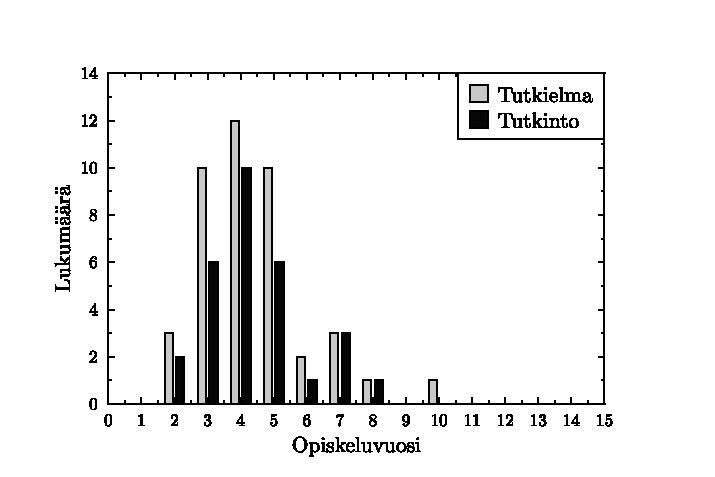
\includegraphics[width=\textwidth]{tutkinnot}
   \caption{Valmistuneiden kandidaatintutkielmien jakauma tekijän opiskeluvuoden mukaan Jyväskylän yliopiston fysiikan laitoksella 2014 ($n = 42$); tutkintojen jakauma opiskeluvuoden mukaan, kun tutkielma on valmistunut 2014 ($n = 29$; tilanne 4.3.2015). (Kuva: Jussi Maunuksela, 2015)}
   \label{fig:esim-kuvio}
\end{figure}

\nocite{*}

% --------------------------------------------------------------------------
% LÄHTEET
% --------------------------------------------------------------------------
%\printbibheading[heading=bibintoc]
\printbibliography
% --------------------------------------------------------------------------
% LIITTEET
% --------------------------------------------------------------------------
\appendix

\section{Appendix 1}
\label{sec:appendix1}
Full guide to manufacturing the chip step by step

\section{Appendix 2}
\label{sec:appendix2}
Arduino code (If i get so far)


\end{document}

